\chapter{The Rendezvous}

The first words that Albert uttered to his friend, on the following
morning, contained a request that Franz would accompany him on a visit
to the count; true, the young man had warmly and energetically thanked
the count on the previous evening; but services such as he had rendered
could never be too often acknowledged. Franz, who seemed attracted by
some invisible influence towards the count, in which terror was
strangely mingled, felt an extreme reluctance to permit his friend to
be exposed alone to the singular fascination that this mysterious
personage seemed to exercise over him, and therefore made no objection
to Albert’s request, but at once accompanied him to the desired spot,
and, after a short delay, the count joined them in the salon.

“My dear count,” said Albert, advancing to meet him, “permit me to
repeat the poor thanks I offered last night, and to assure you that the
remembrance of all I owe to you will never be effaced from my memory;
believe me, as long as I live, I shall never cease to dwell with
grateful recollection on the prompt and important service you rendered
me; and also to remember that to you I am indebted even for my life.”

“My very good friend and excellent neighbor,” replied the count, with a
smile, “you really exaggerate my trifling exertions. You owe me nothing
but some trifle of 20,000 francs, which you have been saved out of your
travelling expenses, so that there is not much of a score between
us;—but you must really permit me to congratulate you on the ease and
unconcern with which you resigned yourself to your fate, and the
perfect indifference you manifested as to the turn events might take.”

“Upon my word,” said Albert, “I deserve no credit for what I could not
help, namely, a determination to take everything as I found it, and to
let those bandits see, that although men get into troublesome scrapes
all over the world, there is no nation but the French that can smile
even in the face of grim Death himself. All that, however, has nothing
to do with my obligations to you, and I now come to ask you whether, in
my own person, my family, or connections, I can in any way serve you?
My father, the Comte de Morcerf, although of Spanish origin, possesses
considerable influence, both at the court of France and Madrid, and I
unhesitatingly place the best services of myself, and all to whom my
life is dear, at your disposal.”

“Monsieur de Morcerf,” replied the count, “your offer, far from
surprising me, is precisely what I expected from you, and I accept it
in the same spirit of hearty sincerity with which it is made;—nay, I
will go still further, and say that I had previously made up my mind to
ask a great favor at your hands.”

“Oh, pray name it.”

“I am wholly a stranger to Paris—it is a city I have never yet seen.”

“Is it possible,” exclaimed Albert, “that you have reached your present
age without visiting the finest capital in the world? I can scarcely
credit it.”

“Nevertheless, it is quite true; still, I agree with you in thinking
that my present ignorance of the first city in Europe is a reproach to
me in every way, and calls for immediate correction; but, in all
probability, I should have performed so important, so necessary a duty,
as that of making myself acquainted with the wonders and beauties of
your justly celebrated capital, had I known any person who would have
introduced me into the fashionable world, but unfortunately I possessed
no acquaintance there, and, of necessity, was compelled to abandon the
idea.”

“So distinguished an individual as yourself,” cried Albert, “could
scarcely have required an introduction.”

“You are most kind; but as regards myself, I can find no merit I
possess, save that, as a millionaire, I might have become a partner in
the speculations of M. Aguado and M. Rothschild; but as my motive in
travelling to your capital would not have been for the pleasure of
dabbling in stocks, I stayed away till some favorable chance should
present itself of carrying my wish into execution. Your offer, however,
smooths all difficulties, and I have only to ask you, my dear M. de
Morcerf” (these words were accompanied by a most peculiar smile),
“whether you undertake, upon my arrival in France, to open to me the
doors of that fashionable world of which I know no more than a Huron or
a native of Cochin-China?”

“Oh, that I do, and with infinite pleasure,” answered Albert; “and so
much the more readily as a letter received this morning from my father
summons me to Paris, in consequence of a treaty of marriage (my dear
Franz, do not smile, I beg of you) with a family of high standing, and
connected with the very cream of Parisian society.”

“Connected by marriage, you mean,” said Franz, laughingly.

“Well, never mind how it is,” answered Albert, “it comes to the same
thing in the end. Perhaps by the time you return to Paris, I shall be
quite a sober, staid father of a family! A most edifying representative
I shall make of all the domestic virtues—don’t you think so? But as
regards your wish to visit our fine city, my dear count, I can only say
that you may command me and mine to any extent you please.”

“Then it is settled,” said the count, “and I give you my solemn
assurance that I only waited an opportunity like the present to realize
plans that I have long meditated.”

Franz did not doubt that these plans were the same concerning which the
count had dropped a few words in the grotto of Monte Cristo, and while
the count was speaking the young man watched him closely, hoping to
read something of his purpose in his face, but his countenance was
inscrutable especially when, as in the present case, it was veiled in a
sphinx-like smile.

“But tell me now, count,” exclaimed Albert, delighted at the idea of
having to chaperon so distinguished a person as Monte Cristo; “tell me
truly whether you are in earnest, or if this project of visiting Paris
is merely one of the chimerical and uncertain air castles of which we
make so many in the course of our lives, but which, like a house built
on the sand, is liable to be blown over by the first puff of wind?”

“I pledge you my honor,” returned the count, “that I mean to do as I
have said; both inclination and positive necessity compel me to visit
Paris.”

“When do you propose going thither?”

“Have you made up your mind when you shall be there yourself?”

“Certainly I have; in a fortnight or three weeks’ time, that is to say,
as fast as I can get there!”

“Nay,” said the Count; “I will give you three months ere I join you;
you see I make an ample allowance for all delays and difficulties.

“And in three months’ time,” said Albert, “you will be at my house?”

“Shall we make a positive appointment for a particular day and hour?”
inquired the count; “only let me warn you that I am proverbial for my
punctilious exactitude in keeping my engagements.”

“Day for day, hour for hour,” said Albert; “that will suit me to a
dot.”

“So be it, then,” replied the count, and extending his hand towards a
calendar, suspended near the chimney-piece, he said, “today is the 21st
of February;” and drawing out his watch, added, “it is exactly
half-past ten o’clock. Now promise me to remember this, and expect me
the 21st of May at the same hour in the forenoon.”

“Capital!” exclaimed Albert; “your breakfast shall be waiting.”

“Where do you live?”

“No. 27, Rue du Helder.”

“Have you bachelor’s apartments there? I hope my coming will not put
you to any inconvenience.”

“I reside in my father’s house, but occupy a pavilion at the farther
side of the courtyard, entirely separated from the main building.”

“Quite sufficient,” replied the count, as, taking out his tablets, he
wrote down “No. 27, Rue du Helder, 21st May, half-past ten in the
morning.”

“Now then,” said the count, returning his tablets to his pocket, “make
yourself perfectly easy; the hand of your time-piece will not be more
accurate in marking the time than myself.”

“Shall I see you again ere my departure?” asked Albert.

“That depends; when do you leave?”

“Tomorrow evening, at five o’clock.”

“In that case I must say adieu to you, as I am compelled to go to
Naples, and shall not return hither before Saturday evening or Sunday
morning. And you, baron,” pursued the count, addressing Franz, “do you
also depart tomorrow?”

“Yes.”

“For France?”

“No, for Venice; I shall remain in Italy for another year or two.”

“Then we shall not meet in Paris?”

“I fear I shall not have that honor.”

“Well, since we must part,” said the count, holding out a hand to each
of the young men, “allow me to wish you both a safe and pleasant
journey.”

It was the first time the hand of Franz had come in contact with that
of the mysterious individual before him, and unconsciously he shuddered
at its touch, for it felt cold and icy as that of a corpse.

\begin{figure}[ht]
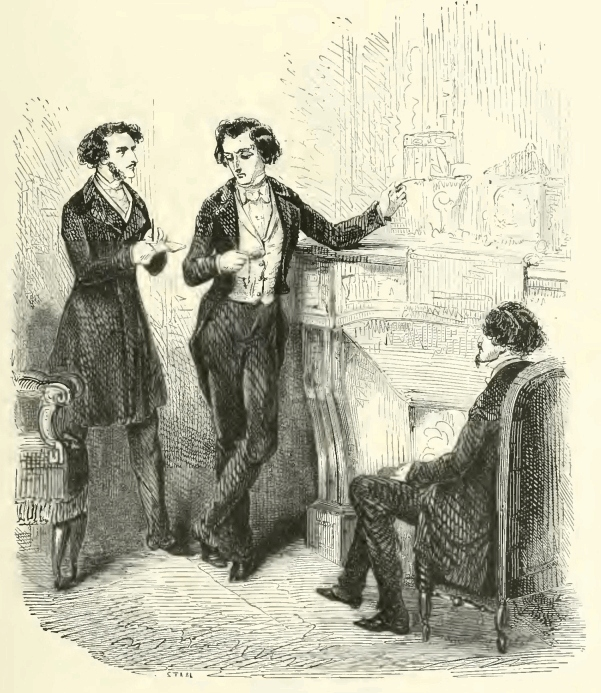
\includegraphics[width=\textwidth]{20219m.jpg}
\end{figure}

“Let us understand each other,” said Albert; “it is agreed—is it
not?—that you are to be at No. 27, in the Rue du Helder, on the 21st of
May, at half-past ten in the morning, and your word of honor passed for
your punctuality?”

“The 21st of May, at half-past ten in the morning, Rue du Helder, No.
27,” replied the count.

The young men then rose, and bowing to the count, quitted the room.

“What is the matter?” asked Albert of Franz, when they had returned to
their own apartments; “you seem more than commonly thoughtful.”

“I will confess to you, Albert,” replied Franz, “the count is a very
singular person, and the appointment you have made to meet him in Paris
fills me with a thousand apprehensions.”

“My dear fellow,” exclaimed Albert, “what can there possibly be in that
to excite uneasiness? Why, you must have lost your senses.”

“Whether I am in my senses or not,” answered Franz, “that is the way I
feel.”

“Listen to me, Franz,” said Albert; “I am glad that the occasion has
presented itself for saying this to you, for I have noticed how cold
you are in your bearing towards the count, while he, on the other hand,
has always been courtesy itself to us. Have you anything particular
against him?”

“Possibly.”

“Did you ever meet him previously to coming hither?”

“I have.”

“And where?”

“Will you promise me not to repeat a single word of what I am about to
tell you?”

“I promise.”

“Upon your honor?”

“Upon my honor.”

“Then listen to me.”

Franz then related to his friend the history of his excursion to the
Island of Monte Cristo and of his finding a party of smugglers there,
and the two Corsican bandits with them. He dwelt with considerable
force and energy on the almost magical hospitality he had received from
the count, and the magnificence of his entertainment in the grotto of
the \textit{Thousand and One Nights}.

He recounted, with circumstantial exactitude, all the particulars of
the supper, the hashish, the statues, the dream, and how, at his
awakening, there remained no proof or trace of all these events, save
the small yacht, seen in the distant horizon driving under full sail
toward Porto-Vecchio.

Then he detailed the conversation overheard by him at the Colosseum,
between the count and Vampa, in which the count had promised to obtain
the release of the bandit Peppino,—an engagement which, as our readers
are aware, he most faithfully fulfilled.

At last he arrived at the adventure of the preceding night, and the
embarrassment in which he found himself placed by not having sufficient
cash by six or seven hundred piastres to make up the sum required, and
finally of his application to the count and the picturesque and
satisfactory result that followed. Albert listened with the most
profound attention.

“Well,” said he, when Franz had concluded, “what do you find to object
to in all you have related? The count is fond of travelling, and, being
rich, possesses a vessel of his own. Go but to Portsmouth or
Southampton, and you will find the harbors crowded with the yachts
belonging to such of the English as can afford the expense, and have
the same liking for this amusement. Now, by way of having a
resting-place during his excursions, avoiding the wretched
cookery—which has been trying its best to poison me during the last
four months, while you have manfully resisted its effects for as many
years,—and obtaining a bed on which it is possible to slumber, Monte
Cristo has furnished for himself a temporary abode where you first
found him; but, to prevent the possibility of the Tuscan government
taking a fancy to his enchanted palace, and thereby depriving him of
the advantages naturally expected from so large an outlay of capital,
he has wisely enough purchased the island, and taken its name. Just ask
yourself, my good fellow, whether there are not many persons of our
acquaintance who assume the names of lands and properties they never in
their lives were masters of?”

“But,” said Franz, “the Corsican bandits that were among the crew of
his vessel?”

“Why, really the thing seems to me simple enough. Nobody knows better
than yourself that the bandits of Corsica are not rogues or thieves,
but purely and simply fugitives, driven by some sinister motive from
their native town or village, and that their fellowship involves no
disgrace or stigma; for my own part, I protest that, should I ever go
to Corsica, my first visit, ere even I presented myself to the mayor or
prefect, should be to the bandits of Colomba, if I could only manage to
find them; for, on my conscience, they are a race of men I admire
greatly.”

“Still,” persisted Franz, “I suppose you will allow that such men as
Vampa and his band are regular villains, who have no other motive than
plunder when they seize your person. How do you explain the influence
the count evidently possessed over those ruffians?”

“My good friend, as in all probability I own my present safety to that
influence, it would ill become me to search too closely into its
source; therefore, instead of condemning him for his intimacy with
outlaws, you must give me leave to excuse any little irregularity there
may be in such a connection; not altogether for preserving my life, for
my own idea was that it never was in much danger, but certainly for
saving me 4,000 piastres, which, being translated, means neither more
nor less than 24,000 livres of our money—a sum at which, most
assuredly, I should never have been estimated in France, proving most
indisputably,” added Albert with a laugh, “that no prophet is honored
in his own country.”

“Talking of countries,” replied Franz, “of what country is the count,
what is his native tongue, whence does he derive his immense fortune,
and what were those events of his early life—a life as marvellous as
unknown—that have tinctured his succeeding years with so dark and
gloomy a misanthropy? Certainly these are questions that, in your
place, I should like to have answered.”

“My dear Franz,” replied Albert, “when, upon receipt of my letter, you
found the necessity of asking the count’s assistance, you promptly went
to him, saying, ‘My friend Albert de Morcerf is in danger; help me to
deliver him.’ Was not that nearly what you said?”

\begin{figure}[ht]
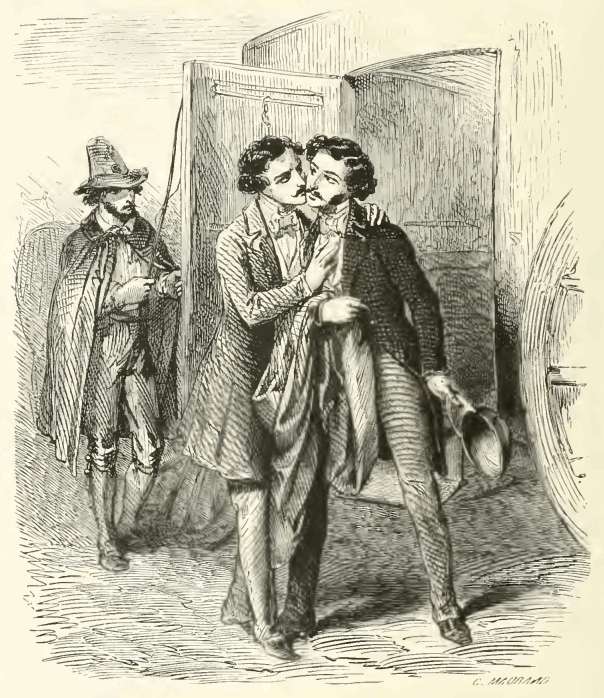
\includegraphics[width=\textwidth]{20222m.jpg}
\end{figure}

“It was.”

“Well, then, did he ask you, ‘Who is M. Albert de Morcerf? how does he
come by his name—his fortune? what are his means of existence? what is
his birthplace? of what country is he a native?’ Tell me, did he put
all these questions to you?”

“I confess he asked me none.”

“No; he merely came and freed me from the hands of Signor Vampa, where,
I can assure you, in spite of all my outward appearance of ease and
unconcern, I did not very particularly care to remain. Now, then,
Franz, when, for services so promptly and unhesitatingly rendered, he
but asks me in return to do for him what is done daily for any Russian
prince or Italian nobleman who may pass through Paris—merely to
introduce him into society—would you have me refuse? My good fellow,
you must have lost your senses to think it possible I could act with
such cold-blooded policy.”

And this time it must be confessed that, contrary to the usual state of
affairs in discussions between the young men, the effective arguments
were all on Albert’s side.

“Well,” said Franz with a sigh, “do as you please my dear viscount, for
your arguments are beyond my powers of refutation. Still, in spite of
all, you must admit that this Count of Monte Cristo is a most singular
personage.”

“He is a philanthropist,” answered the other; “and no doubt his motive
in visiting Paris is to compete for the Monthyon prize, given, as you
are aware, to whoever shall be proved to have most materially advanced
the interests of virtue and humanity. If my vote and interest can
obtain it for him, I will readily give him the one and promise the
other. And now, my dear Franz, let us talk of something else. Come,
shall we take our luncheon, and then pay a last visit to St. Peter’s?”

Franz silently assented; and the following afternoon, at half-past five
o’clock, the young men parted. Albert de Morcerf to return to Paris,
and Franz d’Épinay to pass a fortnight at Venice.

But, ere he entered his travelling carriage, Albert, fearing that his
expected guest might forget the engagement he had entered into, placed
in the care of a waiter at the hotel a card to be delivered to the
Count of Monte Cristo, on which, beneath the name of Viscount Albert de
Morcerf, he had written in pencil:

“27, \textit{Rue du Helder, on the} 21\textit{st May, half-past ten} A.M.”
